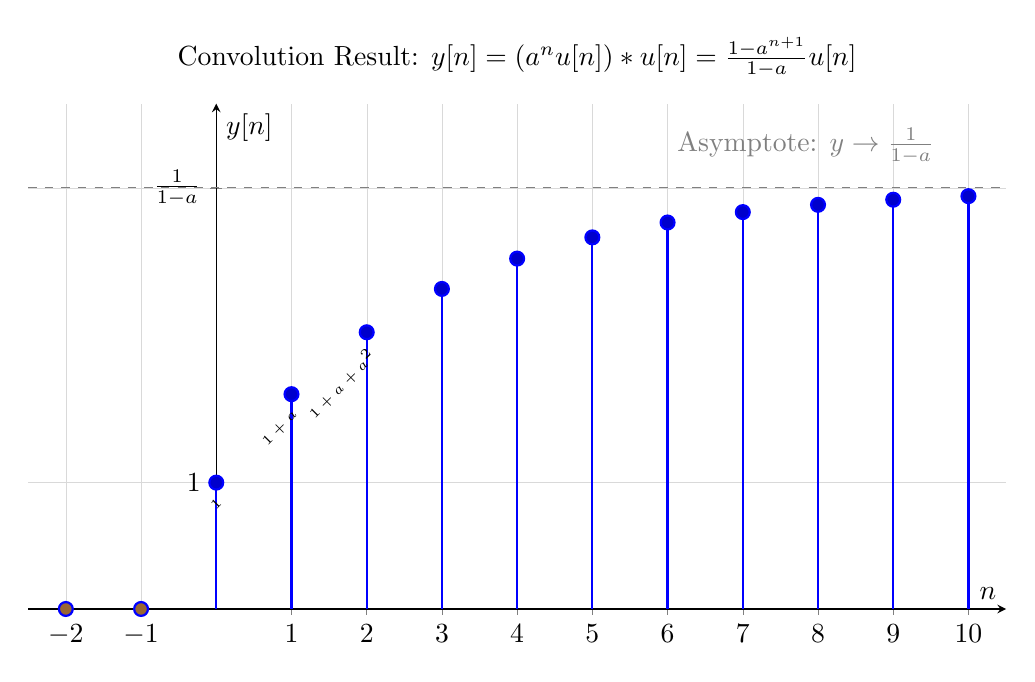
\begin{tikzpicture}
	% Define a style for stem plots
	\pgfplotsset{
		impulse/.style={
			ycomb,
			blue,
			thick,
			mark=*,
			mark size=2.5pt
		}
	}
	
	\begin{axis}[
		width=14cm,
		height=8cm,
		title={Convolution Result: $y[n] = (a^n u[n]) * u[n] = \frac{1-a^{n+1}}{1-a}u[n]$},
		xlabel={$n$},
		ylabel={$y[n]$},
		axis lines=middle,
		xmin=-2.5, xmax=10.5,
		ymin=0, ymax=4,
		xtick={-2,-1,0,1,2,3,4,5,6,7,8,9,10},
		ytick={1,10/3},
		yticklabels={$1$, $\frac{1}{1-a}$},
		grid=major,
		grid style={line width=.1pt, draw=gray!30},
		clip=false,
		]
		
		% Stem plot with custom labels (a = 0.7)
		\addplot+[
		impulse,
		nodes near coords,
		point meta=explicit symbolic,
		every node near coord/.style={
			anchor=north east,
			font=\tiny,
			rotate=45,
			text=black,
		},
		] table [meta=label] {
			x   y         label
			0   1         {$1$}
			1   1.7       {$1+a$}
			2   2.19      {$1+a+a^2$}
			3   2.533     {}
			4   2.7731    {}
			5   2.94117   {}
			6   3.058819  {}
			7   3.1411733 {}
			8   3.1988213 {}
			9   3.2391749 {}
			10  3.2674224 {}
		};
		
		% Horizontal asymptote at y = 1/(1-a) with a=0.7 -> 10/3
		\addplot[dashed, gray, samples=2] coordinates {(-2.5,10/3) (10.5,10/3)};
		\node[anchor=west, gray] at (axis cs:6,11/3) {Asymptote: $y \to \frac{1}{1-a}$};
		
		% Zero-value points to the left
		\addplot+[impulse] coordinates {(-2,0) (-1,0)};
		
	\end{axis}
\end{tikzpicture}
